\subsection{Results of experiments}\label{subsec:resultsofexperiment}
In the experiments, we ran a number of methods on four different datasets that contain either contextual information or side-information.
The methods included two context-aware methods, some state-of-the-art graph-based methods, and some simple baselines.
These methods were evaluated on a number of different metrics that showed their performance on the different datasets.
In this section we look at the results from the experiments.
\begin{figure}[!hbt]
    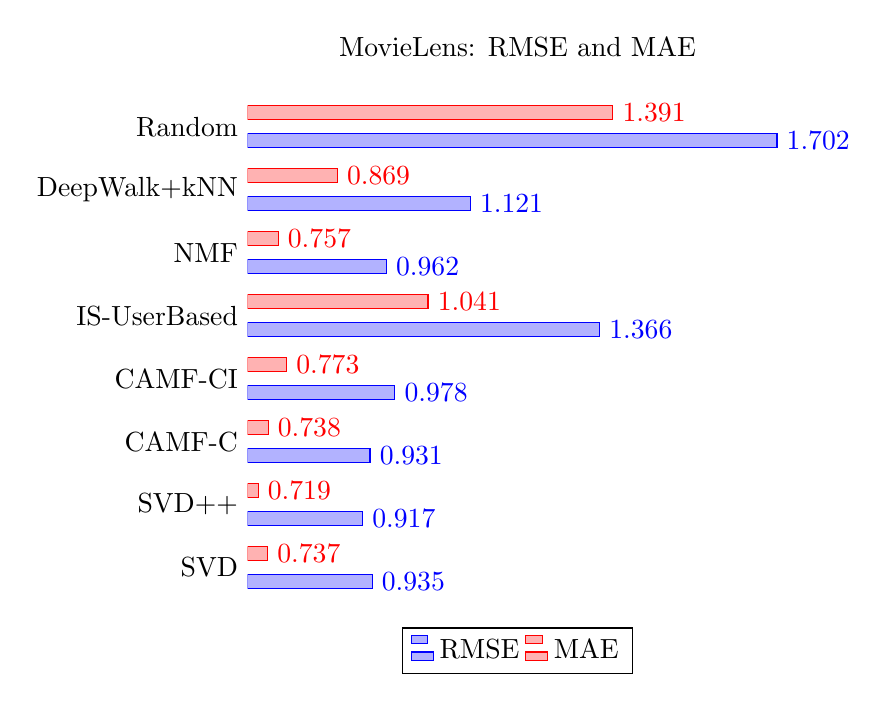
\begin{tikzpicture}
    \begin{axis} [
        title    = {MovieLens: RMSE and MAE},
        xbar=5pt,
        /pgf/bar width=5pt,
        y axis line style = { opacity = 0 },
        axis x line       = none,
        tickwidth         = 0pt,
        enlarge x limits  = 0.02,
        ytick=data,
        y=0.8cm,
        nodes near coords={\pgfmathprintnumber[fixed zerofill, precision=3]{\pgfplotspointmeta}},
        legend style={at={(0.5,-0.03)}, anchor=north,legend columns=-1},
        symbolic y coords = {SVD,SVD++,CAMF-C,CAMF-CI,IS-UserBased,NMF,DeepWalk+kNN,Random},
      ]
    \addplot coordinates{(0.935,SVD) (0.917,SVD++) (0.931,CAMF-C) (0.978,CAMF-CI) (1.366,IS-UserBased) (0.962,NMF) (1.121,DeepWalk+kNN) (1.702,Random)};
    \addplot coordinates{(0.737,SVD) (0.719,SVD++) (0.738,CAMF-C) (0.773,CAMF-CI) (1.041,IS-UserBased) (0.757,NMF) (0.869,DeepWalk+kNN) (1.391,Random)};
    \legend{RMSE,MAE}
    \end{axis}
    \end{tikzpicture}
    \caption{RMSE and MAE results for MovieLens dataset across the investigated methods}
    \label{graph:MLRMSEMAE}
\end{figure}

\begin{figure}[!hbt]
    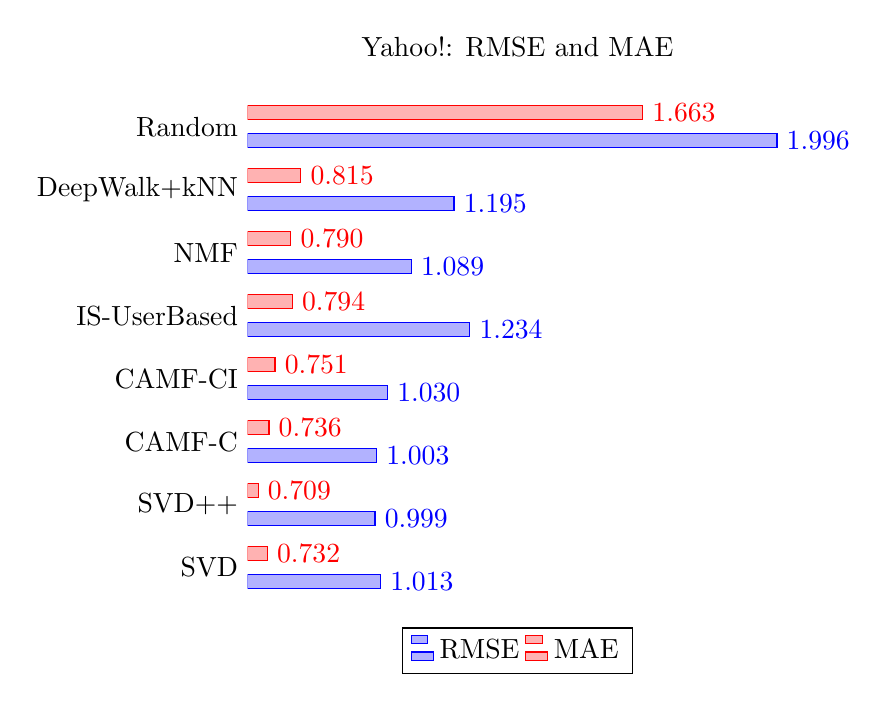
\begin{tikzpicture}
    \begin{axis} [
        title    = {Yahoo!: RMSE and MAE},
        xbar=5pt,
        /pgf/bar width=5pt,
        y axis line style = { opacity = 0 },
        axis x line       = none,
        tickwidth         = 0pt,
        enlarge x limits  = 0.02,
        ytick=data,
        y=0.8cm,
        nodes near coords={\pgfmathprintnumber[fixed zerofill, precision=3]{\pgfplotspointmeta}},
        legend style={at={(0.5,-0.03)}, anchor=north,legend columns=-1},
        symbolic y coords = {SVD,SVD++,CAMF-C,CAMF-CI,IS-UserBased,NMF,DeepWalk+kNN,Random},
      ]
    \addplot coordinates{(1.013,SVD) (0.999,SVD++) (1.003,CAMF-C) (1.030,CAMF-CI) (1.234,IS-UserBased) (1.089,NMF) (1.195,DeepWalk+kNN) (1.996,Random)};
    \addplot coordinates{(0.732,SVD) (0.709,SVD++) (0.736,CAMF-C) (0.751,CAMF-CI) (0.794,IS-UserBased) (0.790,NMF) (0.815,DeepWalk+kNN) (1.663,Random)};
    \legend{RMSE,MAE}
    \end{axis}
    \end{tikzpicture}
    \caption{RMSE and MAE results for Yahoo! dataset across the investigated methods}
    \label{graph:YahooRMSEMAE}
    \end{figure}
    
\begin{figure}[!hbt]
    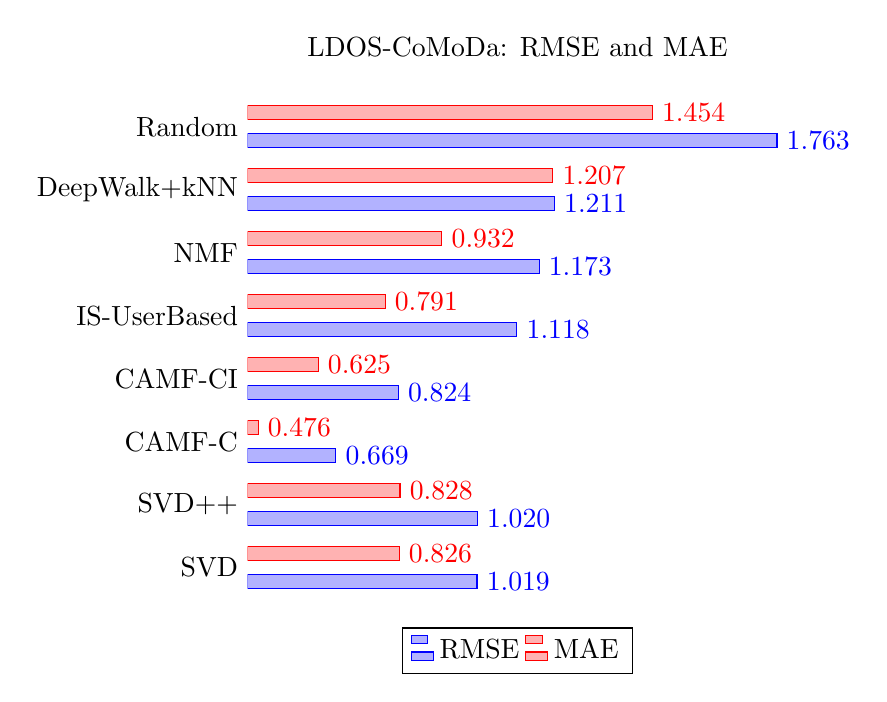
\begin{tikzpicture}
    \begin{axis} [
        title    = {LDOS-CoMoDa: RMSE and MAE},
        xbar=5pt,
        /pgf/bar width=5pt,
        y axis line style = { opacity = 0 },
        axis x line       = none,
        tickwidth         = 0pt,
        enlarge x limits  = 0.02,
        ytick=data,
        y=0.8cm,
        nodes near coords={\pgfmathprintnumber[fixed zerofill, precision=3]{\pgfplotspointmeta}},
        legend style={at={(0.5,-0.03)}, anchor=north,legend columns=-1},
        symbolic y coords = {SVD,SVD++,CAMF-C,CAMF-CI,IS-UserBased,NMF,DeepWalk+kNN,Random},
      ]
    \addplot coordinates{(1.019,SVD) (1.020,SVD++) (0.669,CAMF-C) (0.824,CAMF-CI) (1.118,IS-UserBased) (1.173,NMF) (1.211,DeepWalk+kNN) (1.763,Random)};
    \addplot coordinates{(0.826,SVD) (0.828,SVD++) (0.476,CAMF-C) (0.625,CAMF-CI) (0.791,IS-UserBased) (0.932,NMF) (1.207,DeepWalk+kNN) (1.454,Random)};
    \legend{RMSE,MAE}
    \end{axis}
    \end{tikzpicture}
    \caption{RMSE and MAE results for LDOS-CoMoDa dataset across the investigated methods}
    \label{graph:CoMoDaRMSEMAE}
\end{figure}

\begin{figure}[!hbt]
    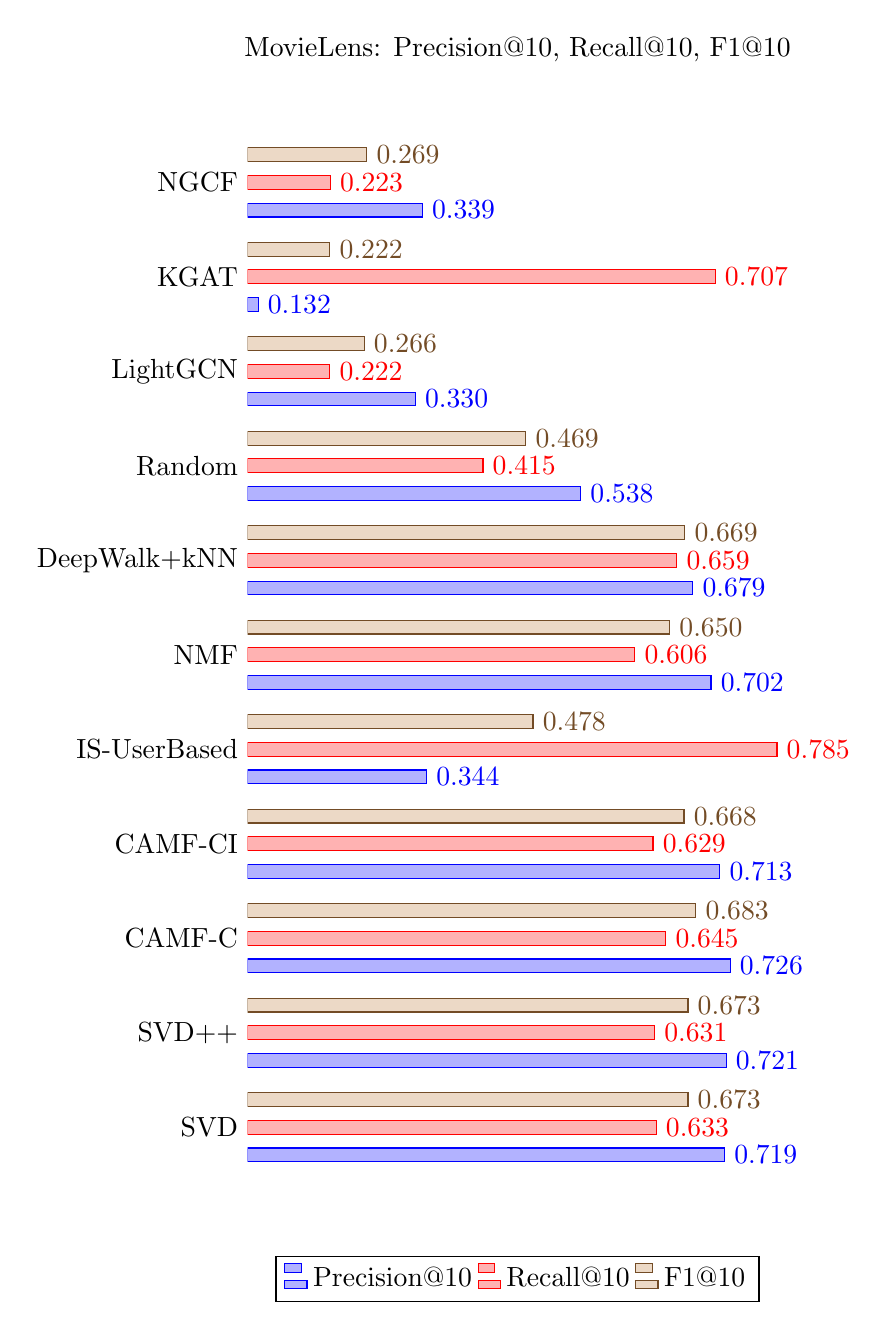
\begin{tikzpicture}
    \begin{axis} [
        title    = {MovieLens: Precision@10, Recall@10, F1@10},
        xbar=5pt,
        /pgf/bar width=5pt,
        y axis line style = { opacity = 0 },
        axis x line       = none,
        tickwidth         = 0pt,
        enlarge x limits  = 0.02,
        ytick=data,
        y=1.2cm,
        nodes near coords={\pgfmathprintnumber[fixed zerofill, precision=3]{\pgfplotspointmeta}},
        legend style={at={(0.5,-0.03)}, anchor=north,legend columns=-1},
        symbolic y coords = {SVD,SVD++,CAMF-C,CAMF-CI,IS-UserBased,NMF,DeepWalk+kNN,Random,LightGCN,KGAT,NGCF},
      ]
    \addplot coordinates{(0.719,SVD) (0.721,SVD++) (0.726,CAMF-C) (0.713,CAMF-CI) (0.344,IS-UserBased) (0.702,NMF) (0.679,DeepWalk+kNN) (0.538,Random) (0.3299,LightGCN) (0.1320,KGAT) (0.3386,NGCF)};
    \addplot coordinates{(0.633,SVD) (0.631,SVD++) (0.645,CAMF-C) (0.629,CAMF-CI) (0.785,IS-UserBased) (0.606,NMF) (0.659,DeepWalk+kNN) (0.415,Random) (0.2222,LightGCN) (0.7072,KGAT) (0.2228,NGCF)};
    \addplot coordinates{(0.673,SVD) (0.673,SVD++) (0.683,CAMF-C) (0.668,CAMF-CI) (0.478,IS-UserBased) (0.650,NMF) (0.669,DeepWalk+kNN) (0.469,Random) (0.265514,LightGCN) (0.222441,KGAT) (0.268757,NGCF)};
    \legend{Precision@10,Recall@10,F1@10}
    \end{axis}
    \end{tikzpicture}
    \caption{Precision@10, Recall@10 and F1@10 results for MovieLens dataset across the investigated methods}
    \label{graph:MLPrecRecF1}
\end{figure}
    
\begin{figure}[!hbt]
    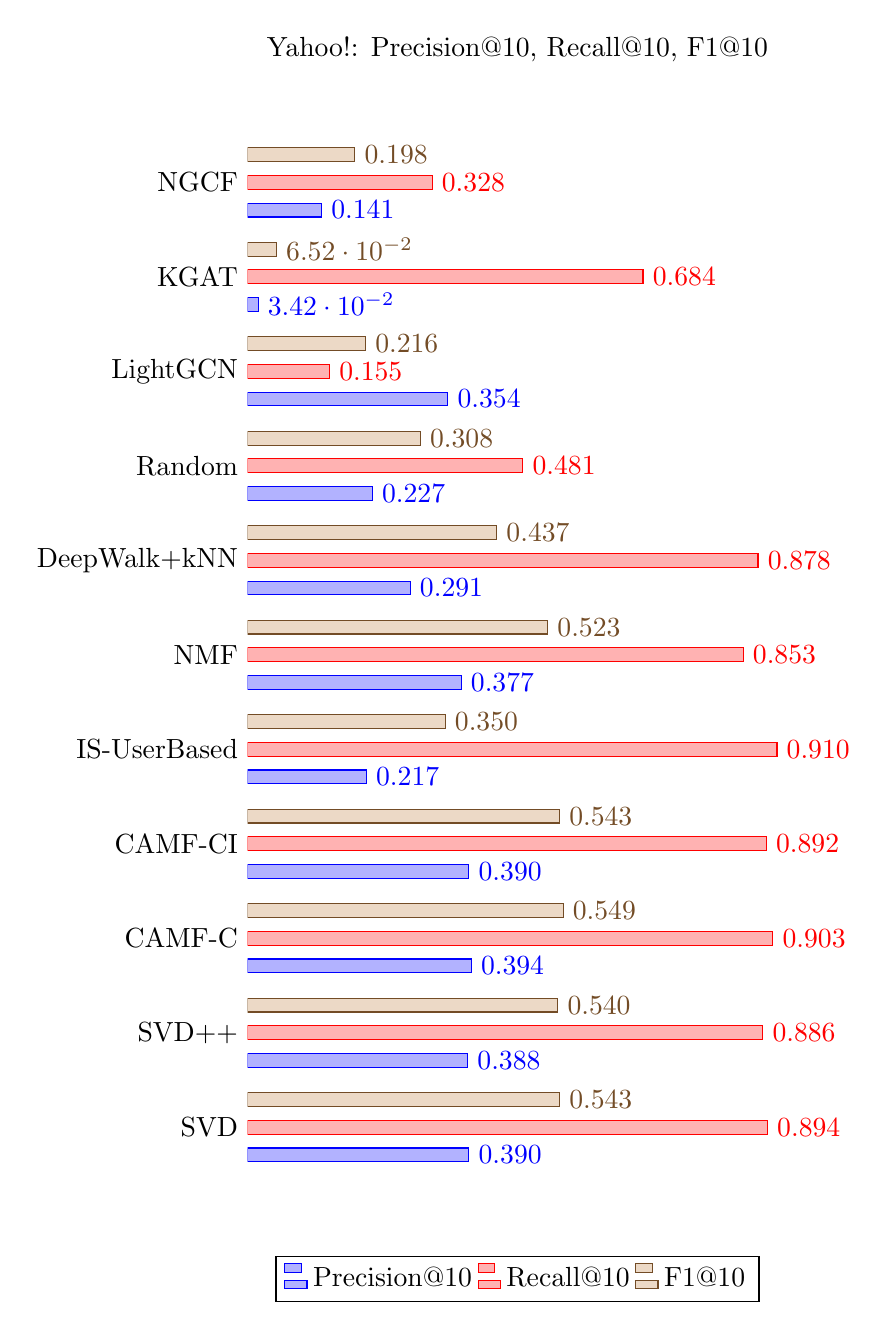
\begin{tikzpicture}
    \begin{axis} [
        title    = {Yahoo!: Precision@10, Recall@10, F1@10},
        xbar=5pt,
        /pgf/bar width=5pt,
        y axis line style = { opacity = 0 },
        axis x line       = none,
        tickwidth         = 0pt,
        enlarge x limits  = 0.02,
        ytick=data,
        y=1.2cm,
        nodes near coords={\pgfmathprintnumber[fixed zerofill, precision=3]{\pgfplotspointmeta}},
        legend style={at={(0.5,-0.03)}, anchor=north,legend columns=-1},
        symbolic y coords = {SVD,SVD++,CAMF-C,CAMF-CI,IS-UserBased,NMF,DeepWalk+kNN,Random,LightGCN,KGAT,NGCF},
      ]
    \addplot coordinates{(0.390,SVD) (0.388,SVD++) (0.394,CAMF-C) (0.390,CAMF-CI) (0.217,IS-UserBased) (0.377,NMF) (0.291,DeepWalk+kNN) (0.227,Random) (0.3544,LightGCN) (0.0342,KGAT) (0.1414,NGCF)};
    \addplot coordinates{(0.894,SVD) (0.886,SVD++) (0.903,CAMF-C) (0.892,CAMF-CI) (0.910,IS-UserBased) (0.853,NMF) (0.878,DeepWalk+kNN) (0.481,Random) (0.1548,LightGCN) (0.6840,KGAT) (0.3280,NGCF)};
    \addplot coordinates{(0.543,SVD) (0.540,SVD++) (0.549,CAMF-C) (0.543,CAMF-CI) (0.350,IS-UserBased) (0.523,NMF) (0.437,DeepWalk+kNN) (0.308,Random) (0.2155,LightGCN) (0.0652,KGAT) (0.1976,NGCF)};
    \legend{Precision@10,Recall@10,F1@10}
    \end{axis}
    \end{tikzpicture}
    \caption{Precision@10, Recall@10 and F1@10 results for Yahoo! dataset across the investigated methods}
    \label{graph:YahooPrecRecF1}
\end{figure}
    
\begin{figure}[!hbt]
    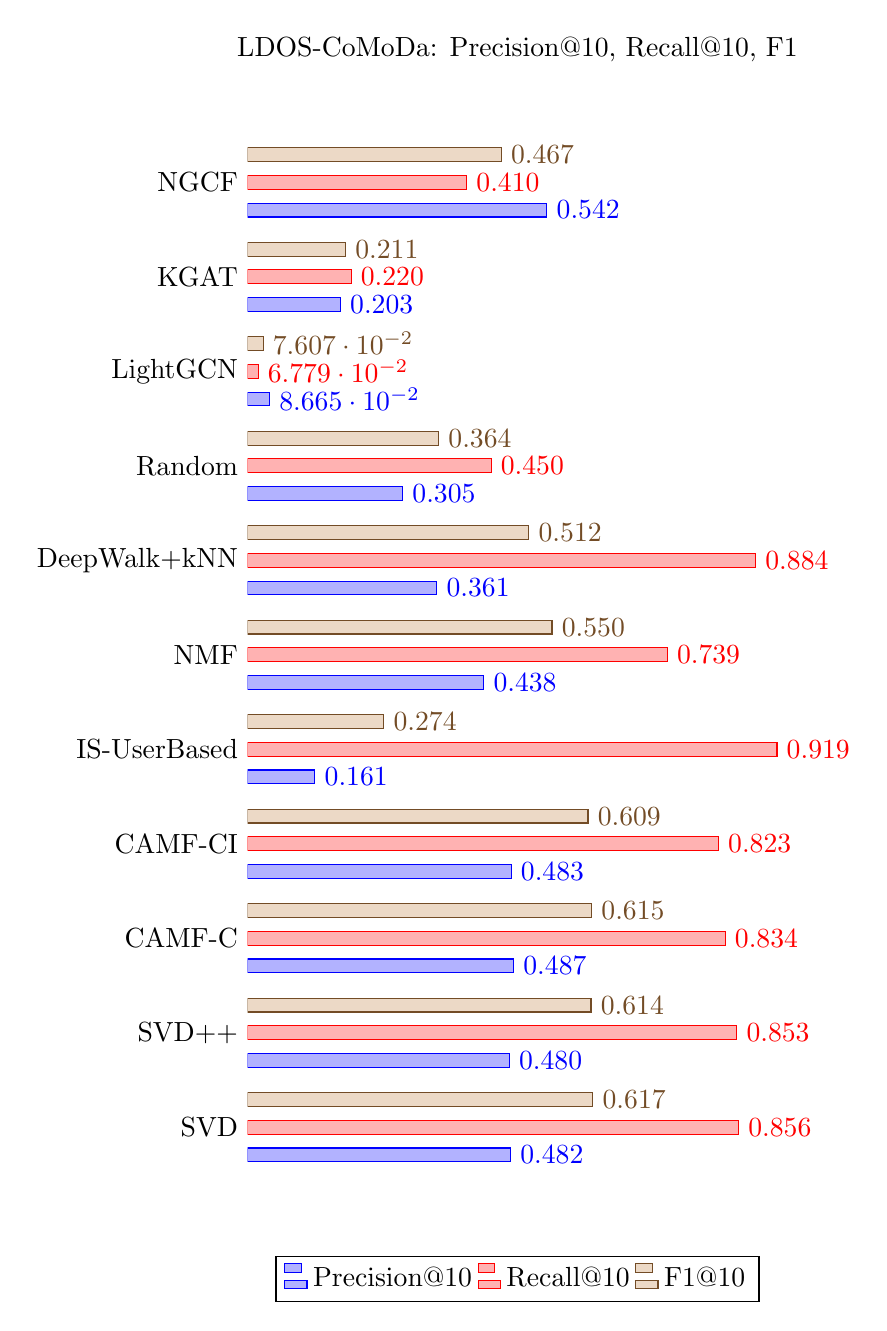
\begin{tikzpicture}
    \begin{axis} [
        title    = {LDOS-CoMoDa: Precision@10, Recall@10, F1},
        xbar=5pt,
        /pgf/bar width=5pt,
        y axis line style = { opacity = 0 },
        axis x line       = none,
        tickwidth         = 0pt,
        enlarge x limits  = 0.02,
        ytick=data,
        y=1.2cm,
        nodes near coords={\pgfmathprintnumber[fixed zerofill, precision=3]{\pgfplotspointmeta}},
        legend style={at={(0.5,-0.03)}, anchor=north,legend columns=-1},
        symbolic y coords = {SVD,SVD++,CAMF-C,CAMF-CI,IS-UserBased,NMF,DeepWalk+kNN,Random,LightGCN,KGAT,NGCF},
      ]
    \addplot coordinates{(0.482,SVD) (0.480,SVD++) (0.487,CAMF-C) (0.483,CAMF-CI) (0.161,IS-UserBased) (0.438,NMF) (0.361,DeepWalk+kNN) (0.305,Random) (0.08665008,LightGCN) (0.20284,KGAT) (0.5416,NGCF)};
    \addplot coordinates{(0.856,SVD) (0.853,SVD++) (0.834,CAMF-C) (0.823,CAMF-CI) (0.919,IS-UserBased) (0.739,NMF) (0.884,DeepWalk+kNN) (0.450,Random) (0.067787792,LightGCN) (0.220396,KGAT) (0.41,NGCF)};
    \addplot coordinates{(0.617,SVD) (0.614,SVD++) (0.615,CAMF-C) (0.609,CAMF-CI) (0.274,IS-UserBased) (0.550,NMF) (0.512,DeepWalk+kNN) (0.364,Random) (0.0760671,LightGCN) (0.211254,KGAT) (0.466700,NGCF)};
    \legend{Precision@10,Recall@10,F1@10}
    \end{axis}
    \end{tikzpicture}
    \caption{Precision@10, Recall@10 and F1@10 results for LDOS-CoMoDa dataset across the investigated methods}
    \label{graph:CoMoDaPrecRecF1}
\end{figure}
    
\begin{figure}[!hbt]
    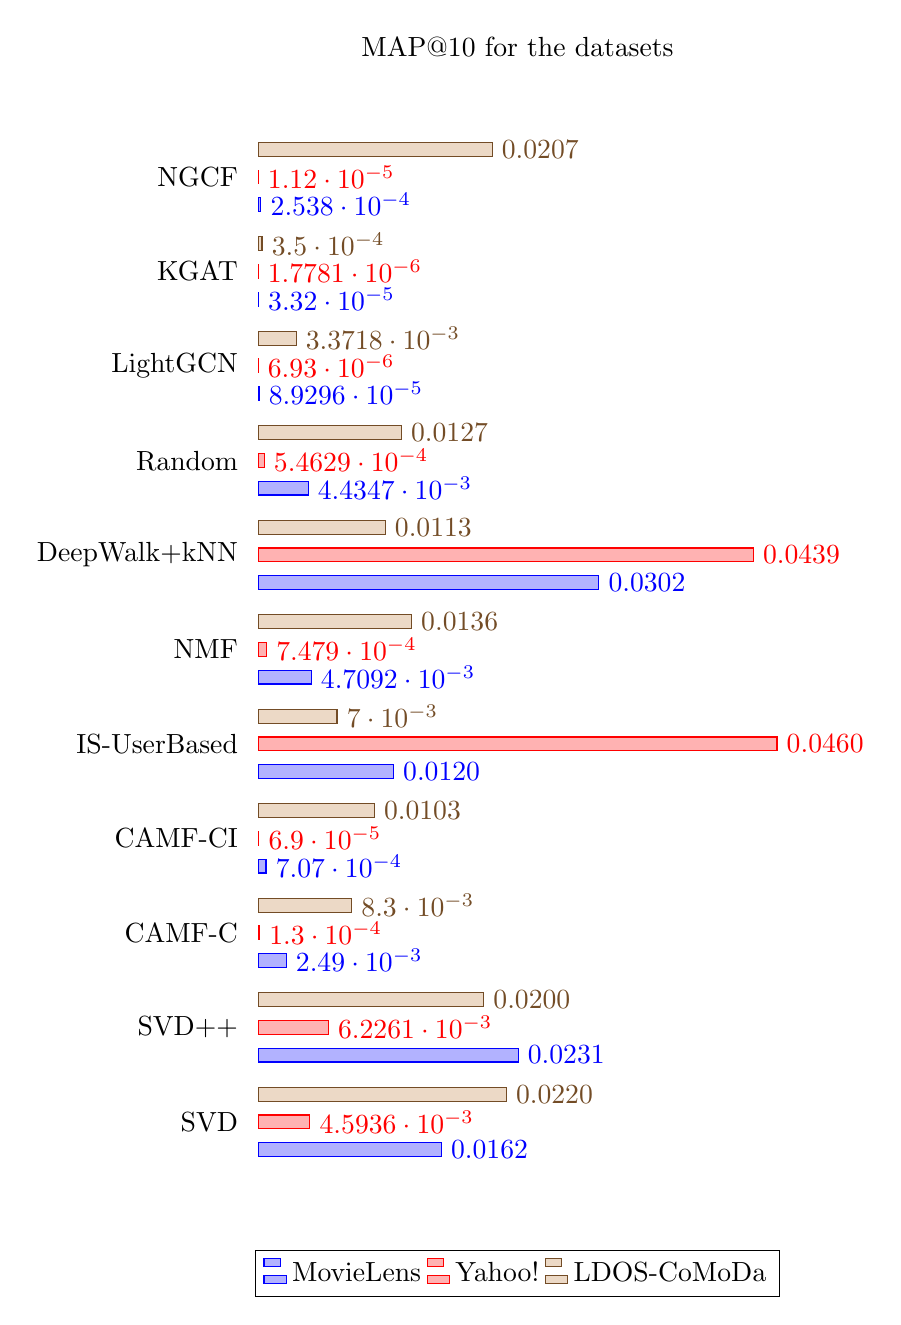
\begin{tikzpicture}
    \begin{axis} [
        title    = {MAP@10 for the datasets},
        xbar=5pt,
        /pgf/bar width=5pt,
        y axis line style = { opacity = 0 },
        axis x line       = none,
        tickwidth         = 0pt,
        enlarge x limits  = 0.02,
        ytick=data,
        y=1.2cm,
        nodes near coords={\pgfmathprintnumber[fixed zerofill, precision=4]{\pgfplotspointmeta}},
        legend style={at={(0.5,-0.03)}, anchor=north,legend columns=-1},
        symbolic y coords = {SVD,SVD++,CAMF-C,CAMF-CI,IS-UserBased,NMF,DeepWalk+kNN,Random,LightGCN,KGAT,NGCF},
      ]
    \addplot coordinates{(0.0162465951248284,SVD) (0.0230514217391177,SVD++) (0.00249,CAMF-C) (0.000707,CAMF-CI) (0.0120,IS-UserBased) (0.00470921880091866,NMF) (0.0302,DeepWalk+kNN) (0.00443467504522534,Random) (0.0000892961875081354,LightGCN) (0.0000332,KGAT) (0.0002538,NGCF)}; % MovieLens
    \addplot coordinates{(0.00459364446058646,SVD) (0.00622607894470324,SVD++) (0.00013,CAMF-C) (0.000069,CAMF-CI) (0.046,IS-UserBased) (0.000747900814877045,NMF) (0.0439,DeepWalk+kNN) (0.000546288347257189,Random) (0.00000693,LightGCN) (0.0000017781423399345,KGAT) (0.0000112,NGCF)}; % Yahoo!
    \addplot coordinates{(0.022,SVD) (0.02,SVD++) (0.0083,CAMF-C) (0.0103,CAMF-CI) (0.007,IS-UserBased) (0.0136,NMF) (0.01127,DeepWalk+kNN) (0.0126990696917064,Random) (0.00337181254,LightGCN) (0.00035,KGAT) (0.020748,NGCF)}; % CoMoDa
    \legend{MovieLens,Yahoo!,LDOS-CoMoDa}
    \end{axis}
    \end{tikzpicture}
    \caption{MAP@10 results for the dataset across the investigated methods}
    \label{graph:MAP10}
\end{figure}
    
\begin{figure}[!hbt]
    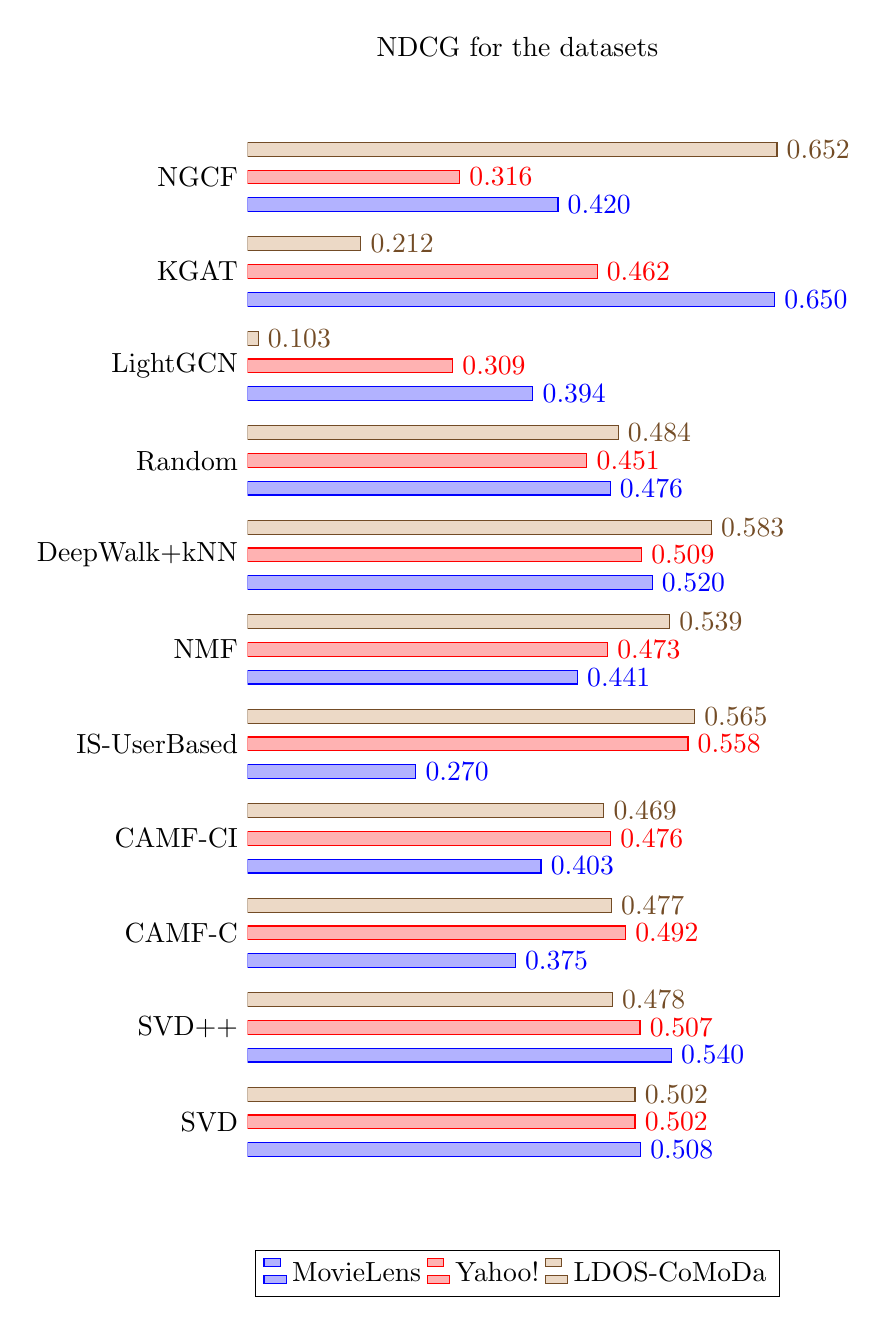
\begin{tikzpicture}
    \begin{axis} [
        title    = {NDCG for the datasets},
        xbar=5pt,
        /pgf/bar width=5pt,
        y axis line style = { opacity = 0 },
        axis x line       = none,
        tickwidth         = 0pt,
        enlarge x limits  = 0.02,
        ytick=data,
        y=1.2cm,
        nodes near coords={\pgfmathprintnumber[fixed zerofill, precision=3]{\pgfplotspointmeta}},
        legend style={at={(0.5,-0.03)}, anchor=north,legend columns=-1},
        symbolic y coords = {SVD,SVD++,CAMF-C,CAMF-CI,IS-UserBased,NMF,DeepWalk+kNN,Random,LightGCN,KGAT,NGCF},
      ]
    \addplot coordinates{(0.507788476243958,SVD) (0.540462250066491,SVD++) (0.3752,CAMF-C) (0.4025,CAMF-CI) (0.270,IS-UserBased) (0.441025641977599,NMF) (0.5201,DeepWalk+kNN) (0.475627993916583,Random) (0.3939,LightGCN) (0.6497,KGAT) (0.4204,NGCF)}; % MovieLens
    \addplot coordinates{(0.501928001717915,SVD) (0.507223962441533,SVD++) (0.492,CAMF-C) (0.476,CAMF-CI) (0.558,IS-UserBased) (0.472880077638768,NMF) (0.5089,DeepWalk+kNN) (0.451040991988228,Random) (0.3090,LightGCN) (0.4618,KGAT) (0.3164,NGCF)}; % Yahoo!
    \addplot coordinates{(0.502,SVD) (0.478,SVD++) (0.477,CAMF-C) (0.469,CAMF-CI) (0.565,IS-UserBased) (0.5385,NMF) (0.5828,DeepWalk+kNN) (0.484100128099788,Random) (0.103,LightGCN) (0.21176,KGAT) (0.6522,NGCF) }; % CoMoDa
    \legend{MovieLens,Yahoo!,LDOS-CoMoDa}
    \end{axis}
    \end{tikzpicture}
    \caption{NDCG@10 results for the dataset across the investigated methods}
    \label{graph:NDCG10}
\end{figure}
\noindent
\autoref{graph:MLRMSEMAE}, \autoref{graph:YahooRMSEMAE} and \autoref{graph:CoMoDaRMSEMAE} visualize RMSE and MAE for MovieLens, Yahoo! and CoMoDa respectively.
Precision@10, Recall@10 and F1@10 are visualized in \autoref{graph:MLPrecRecF1}, \autoref{graph:YahooPrecRecF1} and \autoref{graph:CoMoDaPrecRecF1} for MovieLens, Yahoo! and CoMoDa respectively.
Finally, \autoref{graph:MAP10} visualizes MAP@10 scores for all datasets, while \autoref{graph:NDCG10} visualizes NDCG@10 scores for all datasets.


\subsubsection{LDOS-CoMoDa}
For the experiments conducted on the LDOS-CoMoDa dataset, we should see the methods that handle context do well, as this dataset has many context variables that the rating depends on.
Two of these context variables are used for the experiments, which are the dominantEmo and Physical as these are some of the most influential, as described in \autoref{subsec:desc-of-datasets}.
The methods that handle context are \textit{IS-UserBased} and the \textit{CAMF} methods.
We see that \textit{IS-UserBased} has the largest Recall@10, but also the smallest Precision@10, resulting in a small F1@10 value, and in general, it does not perform well on LDOS-CoMoDa, which is surprising as it is able to utilize the context.
However, \textit{IS-UserBased} is able to achieve one of the highest NDCG@10 scores.
Both \textit{CAMF-C} and \textit{CAMF-CI} perform well on LDOS-CoMoDA in terms of most metrics, except for MAP@N.
They are able to achieve the lowest prediction errors amongst all methods in terms of RMSE and MAE, which could indicate that they are able to make good use of the context.
Close to the results of the \textit{CAMF} methods we have baselines such as \textit{SVD} and \textit{SVD++} which both are competitive in terms of Precision@10, Recall@10 and F1@10. 
These also achieve the highest MAP@10 values but do not have as low prediction errors as the \textit{CAMF} methods.
\textit{NMF} generally performs a little worse in all metrics compared to \textit{SVD}, except for NDCG@10.
The \textit{DeepWalk + kNN} method has high prediction errors and low Precision@10 and MAP@10 values but has the second-highest Recall@10 and one of the highest NDCG@10 values.
Finally, we have the methods that do not handle rating predictions but only do top-$N$ recommendations, so these do not have RMSE and MAE values, since they work with interactions rather than ratings.
We see that \textit{LightGCN} is not able to perform well on any of the metrics.
We suspect that this is because the LDOS-CoMoDa dataset is as small as it is with only 121 users, 1,232 unique movies, and 2,296 ratings, and it is therefore not able to utilize its strengths.
All of these numbers are also lower on the actual data used, due to pruning.
However, \textit{NGCF} is able to achieve both the highest Precision@10 as well as the highest NDCG@10 but does have a lower Recall@10 resulting in a low F1@10 score.
\\\\
To summarize, we expected the context-aware methods to perform well on the LDOS-CoMoDA dataset, as the ratings are context-dependent. 
The \textit{CAMF} methods do perform well as expected, but \textit{IS-UserBased} is underperforming in most metrics.
Some baselines such as \textit{SVD} and \textit{SVD++} are closely competitive with \textit{CAMF} as the best performing methods.
The results of the experiment could also indicate that \textit{NGCF} could be interesting to look at in terms of adding context, as it is able to perform well on a context dataset without utilizing the context available. 
\textit{NGCF} is also a graph-based approach which, as mentioned in \autoref{sec:graph-rec-sys}, is able to alleviate the sparsity problem introduced by adding context.

\subsubsection{MovieLens 100k}
The MovieLens 100k dataset does not contain any contextual variables outside of a timestamp that can be discretized.
\autoref{subsec:experimentprotocol} defined how the timestamp was discretized into the day of the week and a time interval.
Compared to the LDOS-CoMoDa we expected context-aware methods to not perform substantially better since only context based on the timestamp is available compared to the different contextual variables included in the LDOS-CoMoDa dataset. 
In terms of the methods that handle context, we see that \textit{CAMF-C} achieves the highest Precision@10 and F1@10, while \textit{IS-UserBased} underperforms most methods on Precision@10 and outperforms all methods on Recall@10.
In terms of NDCG@10 \textit{IS-UserBased} underperforms on MovieLens compared to other datasets, showing the worst results, while both \textit{CAMF} methods also provide poor NDCG@10.
\textit{KGAT}, a graph-based method utilizing side information performs the best in terms of NDCG@10 on the MovieLens data but underperforms on MAP@10, Precision@10, and F1@10.
Other graph-based methods, such as \textit{NGCF} and \textit{LightGCN} show similar poor performances as well on this dataset, being outperformed on Precision@10, Recall@10, F1@10, and MAP@10.
\textit{DeepWalk} excels on the MAP@10 metric and outperforms other graph-based methods on Precision@10, Recall@10, and F1@10, showing results close to SVD-based approaches.
In terms of RMSE and MAE, we see that both \textit{CAMF} and both \textit{SVD} approaches perform the best, with \textit{Random} underperforming as expected.
Overall, we see a tendency for the graph-based methods to perform poorly on this dataset except for \textit{DeepWalk}, while the SVD-based methods perform the best in terms of F1@10.

\subsubsection{Yahoo! Movies}
For the Yahoo! Movies dataset, we opted to use side-information such as gender and age group as the contextual variables for the context-aware methods since the dataset does not contain any contextual information with the recorded interactions.
Because of this, we do not expect the context-aware methods to perform better than the other baselines.
We see that \textit{SVD++} performs best in terms of RMSE and MAE, closely followed by other methods such as \textit{SVD}, \textit{CAMF}, and \textit{NMF}.
\textit{CAMF-C} is able to achieve the highest Precision@10 which could suggest that it is able to utilize the side information, but it is only marginally better than \textit{SVD}, \textit{SVD++}, and \textit{CAMF-CI}.
For Recall@10, MAP@10, and NDCG@10 \textit{IS-UserBased} is the best performing method.
As this method is context-aware, this could suggest that it is able to improve its predictions using side information.
The high values of MAP@10 and NDCG@10 also suggest that it is better at recommending relevant items in the front of the list compared to other methods.
However \textit{IS-UserBased} does not perform well on Precision@10 nor RMSE and MAE.
\textit{DeepWalk} only performs well on Recall@10, NDCG@10 and MAP@10 and struggles on the other metrics.
\\
In terms of graph-based methods, they do not perform well on this dataset.
\textit{LightGCN}, \textit{NGCF} and \textit{KGAT} all perform evenly in Precision@10, but still show worse results than the methods that are not graph-based.
\textit{LightGCN} shows the best Precision@10 of the graph-based methods, but its Recall@10 and NDCG@10 are worse than many of the baselines.
All of the graph-based methods achieve much worse MAP@10 values than the non-graph-based methods.
\textit{KGAT} has a very low Precision@10 but achieves an NDCG@10 that is comparable to the other baselines.
In general, it does not seem like the graph-based methods are suitable for this kind of dataset.

\subsubsection{Frappé}
The Frappé dataset is a little different, in that it is the only dataset used without ratings, focusing solely on interactions.
As such, only results from methods that are able to produce a top-$N$ list are reported.
For Precision@10 we see that \textit{LightGCN} outperforms the others, and \textit{NGCF} shows poor performance on the metric compared to both \textit{LightGCN} and \textit{KGAT}.
For Recall@10 however, \textit{KGAT} shows the best performance by a substantial amount, whereas \textit{LightGCN} and \textit{NGCF} perform mostly evenly.
\textit{KGAT}'s overall performance on Precision@10 and Recall@10 lead to it performing the best on F1@10, where \textit{LightGCN} also outperforms \textit{NGCF}.
For these metrics, we see that the random baseline performs substantially worse than the state-of-the-art methods.
\textit{KGAT} outperforms the other methods except for random on NDCG@10, while performing poorly on MAP@10, which \textit{NGCF} performs the best on with the exception of random that surprisingly performs decently on the MAP@10 metric.
